\documentclass[a4paper, notitlepage]{article}
\usepackage{fullpage}
\usepackage[utf8]{inputenc}
\usepackage{tikz}
\usetikzlibrary{automata,positioning}
\DeclareUnicodeCharacter{9251}{\openboxtest}
\begin{document}

\makeatletter
\renewcommand\paragraph{\@startsection{paragraph}{4}{\z@}%
  {-3.25ex\@plus -1ex \@minus -.2ex}%
  {1.5ex \@plus .2ex}%
  {\normalfont\normalsize\bfseries}}
\makeatother

\title{TI2320 Theory of Computation, assignment 2 (ndtm-2)} 
\author{Zmitser Zhaleznichenka (\#4134575, group 39)}
\date{\today}
\maketitle

\setcounter{secnumdepth}{0}

\section{Task 1}

\subsection{Algorithm idea}

The Turing machine has to check for a given graph $G = (V, E)$ whether it has a spanning tree $T$ with the set of leaves equal to the given set of nodes $L \subseteq V$. To do so, we use the following algorithm.

\begin{enumerate}
\item Check whether $G$ is properly described and connected: a disconnected graph doesn't have a spanning tree.
\item For each node in $L$ find a set of directly connected neighbors $N : N_i \notin L$. If any $N_{L_i} = \emptyset$, reject, as in this case two leaves from a set have to be connected.
\item For each node in $L$ select the first neighbor from $N_{L_i}$, form a set $I$ from the selected nodes. 
\item If graph $G' = (I, E_0)$ is connected, accept. Otherwise, go to step 3 and create the next set $I$. If no one set is connected, reject.
\end{enumerate}

With such an algorithm we ensure that every node in $L$ has a degree 1, which makes these nodes the leaves of the spanning tree. If the rest of the nodes can be connected, there is a spanning tree in graph $G'$. If we add the nodes from $L$ to this spanning tree with the edges chosen at step 3, we get a spanning tree for $G$ and will not introduce the new leaves.

The graph should be modeled as explained in example 3.23 at Sipser.

\subsection{Implementation details}

\paragraph{Checking graph G for correct representation and connectivity}

Refer to example 3.23 at Sipser.

\paragraph{Generating set of neighbor nodes and verifying their state}

\begin{enumerate}
\item Assume the graph representation is stored at tape A, set $L$ is stored at tape B. Take an empty tape C.
\item For all the nodes $L_i$ in $L$ go through graph representation at A to find nodes adjacent to $L_i$ (they form the edges with $L_i$). Copy all such nodes that are not in $L$ to C and separate the neighbor sets for different nodes with \#.
\item If the string in C has two or more consequent \#s, reject (empty set of neighbors for at least one leaf).
\item Mark every first node in every set in C separated by \# with a dot.
\item Copy all the unique nodes from C marked with a dot to a clean tape D. 
\item Copy all the edges between nodes in D from A to D. Now we have a representation of graph $G'$ at tape D. 
\item Check $G'$ for connectivity as it is done for graph $G$. If it is connected, accept.
\item Clear D. Move the last dot in C to the right. If it is already in rightmost position, move it to the first position after the \# and move the preceding dot to the right. If the first dot is moved from the rightmost position to the left, reject. Otherwise go to step 5.
\end{enumerate}

\subsection{State diagram for a non-deterministic choice}

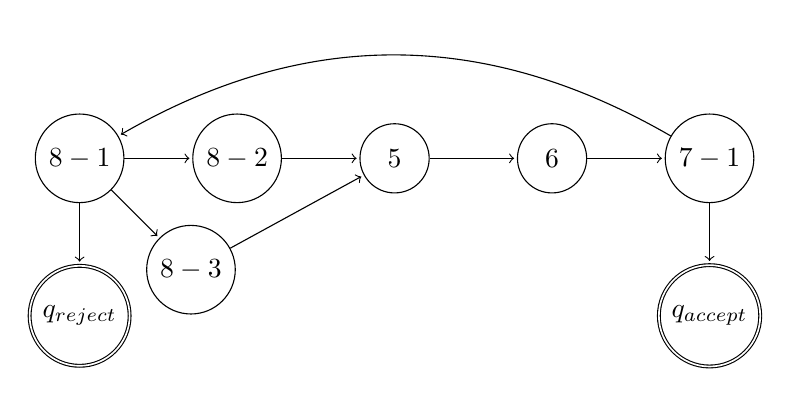
\begin{tikzpicture}[shorten >= 1pt, node distance=2cm,on grid,auto]
\node[state](q_81){$8-1$};
\node[state](q_82) [right=of q_81]{$8-2$};
\node[state](q_83) [below right=of q_81]{$8-3$};
\node[state, accepting](q_84) [below=of q_81]{$q_{reject}$};
\node[state](q_5) [right=of q_82]{$5$};
\node[state](q_6) [right=of q_5]{$6$};
\node[state](q_71) [right=of q_6]{$7-1$};
\node[state, accepting](q_72) [below=of q_71]{$q_{accept}$};
\path[->]
(q_81) edge node {} (q_82)
	 edge node {} (q_83)
 	 edge node {} (q_84)
(q_82) edge node {} (q_5)
(q_83) edge node {} (q_5)
(q_5) edge node {} (q_6)
(q_6) edge node {} (q_71)
(q_71) edge node {} (q_72)
(q_71) edge [bend right] node {} (q_81);
\end{tikzpicture}
\newline\newline
Here we see the state diagram for steps 5-8 of the algorithm above. In state $8-1$, we have to find the position of last dot in the neighbor set and move it to the right. There are several different options. First, if we can move the last dot to the right, we do it by moving to state $8-2$. If the last dot is already at the rightmost place and we have to adjust the preceding dots, we move to state $8-3$. And lastly, if all the dots are at their rightmost positions, we move to state $q_{reject}$ that indicates that we have checked all the possible combinations from the neighbors superset and have to halt with \emph{reject}. From either of states $8-2$ and $8-3$ we can proceed to step 5 and further, and eventually reach accepting state $q_{accept}$ which means that we have found a connected set of neighbors.

\section{Task 2}

In $G = (V,E)$ we have $n$ vertices and $m_n$ edges with $m_n \le n(n-1)/2$. To check $G$ for connectivity, we need to perform at most $n^2*m_n$ operations, as follows from 3.23 exercise algorithm analysis. 

It takes $|L|*m_n$ time to build neighbor sets for all the nodes in $L$, so at most $n*m_n$ operations if $|L| = n$.

At most $n - |L|$ nodes may form sets of neighbors, which gives us $2^{n - |L|}$ different neighbors sets to consider, this is at most $2^{n-2}$. Each of these sets has to be checked for connectivity, which can be done in $k^2*m'$ time, where $k$ is the number of nodes in this neighbor set, $m'$ is the number of edges in the set.

Thus, the total formula is $f(n) = n^2*m_n + n*m_n + 2^{n-2}*(n-2)^2*m_{n-2}$. $T(f(n)) = O(2^n).$


\end{document}